%%%% Proceedings format for most of ACM conferences (with the exceptions listed below) and all ICPS volumes.
\newif\ifanon\anontrue
\documentclass[sigconf,anonymous]{acmart}
\usepackage{paralist}
\usepackage{url}
\usepackage[hyphenbreaks]{breakurl}

\def\UrlBreaks{\do\/\do-}

%%%% As of March 2017, [siggraph] is no longer used. Please use sigconf (above) for SIGGRAPH conferences.

%%%% Proceedings format for SIGPLAN conferences 
% \documentclass[sigplan, anonymous, review]{acmart}

%%%% Proceedings format for SIGCHI conferences
% \documentclass[sigchi, review]{acmart}

\usepackage{booktabs} % For formal tables


% Copyright
%\setcopyright{none}
%\setcopyright{acmcopyright}
\setcopyright{acmlicensed}
%\setcopyright{rightsretained}
%\setcopyright{usgov}
%\setcopyright{usgovmixed}
%\setcopyright{cagov}
%\setcopyright{cagovmixed}

\copyrightyear{2019}
\acmYear{2019}
\setcopyright{acmlicensed}
\acmConference[CompEd 2019]{The ACM Global Computing Education
  Conference 2019}{Mar. 17--19, 2019}{Chengdu, China}
%\acmBooktitle{}
%\acmPrice{15.00}
%\acmDOI{10.1145/3159450.3159547}
%\acmISBN{978-1-4503-5103-4/18/02}
% This slight change to the code may also save 1 or 2 lines of space.

% removes the headers from each page per the preparation instructions, as these are not needed and will be updated with the chairs' actual session names during the pagination/indexing process:
\fancyhead{}

\begin{document}
\title{The Institute of Coding: A University-Industry Collaboration to Address the UK Digital Skills Crisis}
%\titlenote{}
%\subtitle{Extended Abstract}
%\subtitlenote{}
\author{James H. Davenport}
\orcid{0000-0002-3982-7545}
\affiliation{%
  \institution{University of Bath}
  \streetaddress{}
  \city{Bath} 
  \country{United Kingdom}
}
\email{j.h.davenport@bath.ac.uk}

\author{Tom Crick}
\orcid{0000-0001-5196-9389}
\affiliation{%
  \institution{Swansea University}
  \streetaddress{}
  \city{Swansea} 
  \country{United Kingdom}
}
\email{thomas.crick@swansea.ac.uk}

\author{Alan Hayes}
%\orcid{}
\affiliation{%
  \institution{University of Bath}
  \streetaddress{}
  \city{Bath} 
  \country{United Kingdom}
}
\email{a.hayes@bath.ac.uk}

\author{Rachid Hourizi}
%\orcid{}
\affiliation{%
  \institution{University of Bath}
  \streetaddress{}
  \city{Bath} 
  \country{United Kingdom}
}
\email{r.hourizi@bath.ac.uk}
 
% The default list of authors is too long for headers}

\renewcommand{\shortauthors}{Davenport, Crick, Hayes and Hourizi}


\begin{abstract}
The Institute of Coding is a new \pounds40m+ initiative by the UK
Government to ``transform the digital skills profile of the
country''. In the context of significant national and international
policy scrutiny, it responds to the apparently contradictory data that
the country has a digital skills shortage across a variety of sectors,
yet the Higher Education system produced computing graduates every year who end up unemployed, or underunemployed.

 The Institute is a large-scale national intervention to address some of the perceived
issues with formal education versus industry skills and training, for
example: technical skills versus soft skills, industry-readiness
versus ``deep education'', and managing expectations for the diverse
digital, data and computational skills demands of employers across a
wide range of economic sectors.

All of this is taking place in the higher education/workforce domain
at the same time as substantial levels of computer science curriculum
reform across the four nations of the UK -- especially in England,
with a new computing curriculum that first started in 2014, in which
all children are expected to learn two programming languages, as well
as wider computer science fundamentals and develop transferability
computational thinking skills.

In this paper, we describe the background and evidence base for the
Institute of Coding, its key themes and current activities, as well as
reflecting on potential replicability of aspects of the Institute (and
related initiatives in the UK) to other nations or regions with
similar ambitions to address the ``digital skills crisis''.
%its hybrid structure, key themes and planned deliverables, identifying some of the key opportunities and challenges, as well as its potential replicability of aspects of the Institute in other jurisdictions.
\end{abstract}

\begin{CCSXML}
<ccs2012>
<concept>
<concept_id>10003456.10003457.10003527.10003531.10003533</concept_id>
<concept_desc>Social and professional topics~Computer science education</concept_desc>
<concept_significance>500</concept_significance>
</concept>
<concept>
<concept_id>10003456.10003457.10003527.10003531.10003535</concept_id>
<concept_desc>Social and professional topics~Information technology education</concept_desc>
<concept_significance>500</concept_significance>
</concept>
<concept>
<concept_id>10003456.10003457.10003527.10003531.10003751</concept_id>
<concept_desc>Social and professional topics~Software engineering education</concept_desc>
<concept_significance>500</concept_significance>
</concept>
<concept>
<concept_id>10003456.10003457.10003580.10003568</concept_id>
<concept_desc>Social and professional topics~Employment issues</concept_desc>
<concept_significance>500</concept_significance>
</concept>
<concept>
<concept_id>10003456.10003457.10003458</concept_id>
<concept_desc>Social and professional topics~Computing industry</concept_desc>
<concept_significance>300</concept_significance>
</concept>
</ccs2012>
\end{CCSXML}

\ccsdesc[500]{Social and professional topics~Computer science education}
\ccsdesc[500]{Social and professional topics~Information technology education}
\ccsdesc[500]{Social and professional topics~Software engineering education}
\ccsdesc[500]{Social and professional topics~Employment issues}
\ccsdesc[300]{Social and professional topics~Computing industry}

\keywords{Digital skills, Programming, Computer science education,
  Undergraduate education, Graduate education, Industry collaboration, UK}   %JHD True, but is it worth a line?

\maketitle

% From CfP:
% Short papers (up to 5 pages) focus on dissemination and discussion
% of new ideas in computing education practice or research that merit
% wider awareness and discussion within the community. They can present
% preliminary results of new educational innovations, present and
% discuss novel educational technologies, report work-in-progress
% research (including promising systems or tools that have not yet been
% evaluated and/or adopted extensively), or raise issues of significance
% for the development of the discipline, such as long-term strategic
% needs for computing education and curricula. All short papers are
% expected to have an appropriate coverage of literature to support the
% ideas and arguments that they present. Because it lacks some elements
% of a research paper, a short paper is evaluated mainly by its
% anticipated impact on discussions during the conference and possible
% future contribution to the field of computing education.

\section{Introduction}

% TC: need more UK context here, I can add this -- do we want to have
% this framed as a paper to justify/introduce the IoC, as well as
% other UK interventions? Framed as a discussion piece with
% transferability elsewhere?
%Set the scene -- UK digital skills, CS ed reform, digital economy, etc

We are frequently being told that this is ``the digital age'', and
that we ``live in a knowledge economy''\footnote{Despite the debunking
  in \cite{Friesen2008}.}
, with ``software eating the
world''~\cite{andreessen:2011}; nevertheless, the impact of digital on all of our
lives is clear. From entertainment and communication, via the power
and reach of an oligopoly of social media platforms, with ``algorithms''
influencing what we see or making decisions that affect us every day;
to education, health and social care, and innovation in public
services~\cite{ecdsmsuk:2018}.

\subsection{Defining the ``Digital Economy''}

Providing a comprehensive definition of the `digital economy' is
challenging; the OECD's 2002 definition of the ICT sector does not
provide much insight: ``{\emph{...a combination of manufacturing and
services industries that capture, transmit and display data and
information electronically}}''~\cite{oecd:2002}.  According to the
2007 UK Standard Industrial Classification of Economic
Activities~\cite{onssic:2009}, the ``Information and Communication''
sector includes telecommunications, computer programming, information
services, as well as a wide range of creative, publishing and
broadcasting activities. Formal sector classifications aside, it is
clear that while we may the UK may have a traditional vertical `IT and
Telecoms' sector, we also have a crucial enabling and facilitative
horizontal digital sector -- in essence: there is no such thing as the
`digital economy' -- our economy is digital. While this situation is
not unique to the UK, it is perhaps exemplified by some of the grand
challenges identified as part of the 2017 UK Industrial
Strategy~\cite{ukis:2017}: from precision medicine, manufacturing and
future materials, to creative industries clusters and next generation
services, through to driverless cars and smart
cities~\cite{tryfonas+crick:petra2018}.

\subsection{Diversity, especially Gender}\label{sec:Gender}

In 2017, the UK digital sector comprised of 1.5 million jobs (4.6\% of
the total number of jobs in the UK), the highest number for the sector
(and a 16.1\% increase) since 2011~\cite{dcms:2017}. Its workers are
more productive, on average, by \pounds10,000 per worker and jobs
requiring digital tech skills command higher salaries, at
\pounds42,578 compared to \pounds32,477 for those that do not. Despite
the stereotype that digital tech jobs are for ``millennials'', 72\% of
workers are aged over 35; however, only 19\% of the UK digital tech
workforce is female~\cite{technation:2018}. Indeed, the Institute of
Coding announcement \cite{DfE2018a} quoted the even more pessimistic
``In 2017, female programmers and software developers made up just 3.9
per cent of tech and telco professionals in the UK''.

\subsection{Education and Skills Policy}

Across the world there are a plethora of initiatives and interventions
to address the wider societal challenge, and the corresponding skills
shortages~\cite{cece:2017}. While there is a strong socio-economic
policy focus, it should not just be about jobs: we want, and need, a
digitally competent, capable and engaged citizenry. But what do we
mean by digital skills? In recent years, we have seen a multitude of
policy reviews and reports from across government, academia, think
tanks, learned societies and charities that have attempted to
encapsulate some of the issues, as well as identifying potential
solutions. At least three recent UK Parliament Select Committee
inquiries~\cite{ukholds:2015,ukhocst:2016,ukholc:2017} have, wholly or
in part, focused on the `digital skills crisis'. They have made a
number of specific recommendations, from curriculum and qualifications
reform, improving professional learning for practitioners, investment
in infrastructure, developing effective pedagogies and the wider
educational research base in the UK, through to terminology, fixing
`leaky pipelines' and changing wider public perceptions of the
discipline.

Alongside substantial curriculum reform across the
%UK~\cite{crick+sentance:2011,brown-et-al:sigcse2013,brown-et-al:toce2014},
UK~\cite{brown-et-al:sigcse2013,brown-et-al:toce2014},
including a new national curriculum in England~\cite{DfE2013a} and
emerging reform in
%Wales~\cite{wgictreview:2013,crick+moller:wipsce2015,moller+crick:jce2018},
Wales~\cite{wgictreview:2013,moller+crick:jce2018},
we have also seen significant changes to the available qualifications,
based on perceived rigour, content, distinctiveness and modes of
assessment. The publication last year of a follow-up report on
computing education in the UK from the Royal Society~\cite{rs:2017}
framed some of these national challenges in the context of computing
for all, calling for a coherent strategy so that all learners are
equipped and empowered with the necessary skills to be effective in
the digital world.

However, it is clear that from all of these various reviews, reports,
activities, initiatives and interventions, there remains a lack of
connectedness and policy coherency -- more so when it cuts across
ministerial portfolios, or requires multi-year coordinated support. In
this paper we frame some of these discrete challenges -- and
opportunities -- and introduce the Institute of Coding, a new
\pounds40m+ initiative by the UK Government (but focused on
England, with related activity in Wales) to transform the digital
skills profile of the country.

The structure of the paper is as follows. In Section~\ref{problem} we
attempt to define the wider problem through the lens of graduate
employment and earnings; this is followed in Sections~\ref{ukhepolicy}
and~\ref{sec:Skills} by the UK higher education policy context and the
skills mismatch respectively; in Section~\ref{ioc} we present the
Institute of Coding and its key themes and activities, finishing with
future work and the potential replicability of aspects of
the Institute in Section~\ref{concl}.

% and now in Lithuania \cite{Xinhua2018a}) to prisons \cite{Maher2018a}.

\subsubsection*{A Note on Nomenclature}

While in many instances throughout this paper we will refer to the
United Kingdom (UK) -- consisting of the four nations of England,
Scotland, Wales and Northern Ireland -- many of the %specific
initiatives, approaches and funding models are specifically focused on
England (or England and Wales) as a number of policy areas,
including education and skills, are devolved to the respective
governments. We will attempt to be as clear as possible when referring
to specific interventions across or between the four nations.

\section{So What's the Problem?}\label{problem}

Superficially, the employment outlook for computing graduates in the
UK looks excellent. \cite[p.~74]{UKCES2015b} states
\begin{quote} the digital sub-sector will need 518,000 workers for
roles in the three highest skilled occupational groups. However, over
the last ten years only 164,000 individuals graduated from a first
degree in computer science.
\end{quote} This is profitable for the individual: according to
\cite[Figure 4]{BIS2011a}, ``mathematical and computer sciences'' have
the second highest earnings return of all subjects (beaten only by
``medicine and dentistry'').  The country profits from this as well:
according to \cite[p.~16]{BIS2011a}, this is, per head, the fourth
most beneficial subject to the UK.
Despite the headline success in \cite{BIS2011a}, the employment
figures are not great, and the earnings data are patchy.

\subsection{Graduate Employment}

Quoting \cite{UKCES2015b}, the author of a UK Government-commissioned
report \cite{Shadbolt2016a} writes:

\begin{quote} In this context, apparently high rates of
unemployment\footnote{11.7\% six months after graduation (the standard
UK measure) at the time of \cite{Shadbolt2016a}, compared with a STEM
average of 8.4\%. Note, however, that Computing is 20\% of STEM
\cite[Table 1]{Wakeham2016a}, so `STEM-less-Computing' has a 7.6\%
unemployment rate.} amongst graduates of Computer Sciences and other
STEM\footnote{STEM is ``Science, Technology, Engineering,
Mathematics'' for \cite{Shadbolt2016a} and this paper.} courses
demanded an explanation.
\end{quote}

A significant explanation is ``There are notable differences in the
characteristics of Computer Sciences entrants compared to entrants in
other STEM subjects'' \cite[\P2.6]{Shadbolt2016a}: fewer women, but

\begin{description}
\item[50\% more] mature students,
\item[16\% more] Black and Minority Ethnic (BME) and
\item[40\% more] students from backgrounds where people have
traditionally not participated in HE (low participation
neighbourhoods, LPNs).
\end{description}

Mature, BME and LPN students all find getting jobs more difficult.
\par However, for those students that do find jobs, the data are
better, showing \cite[Figure 6]{Shadbolt2016a} fewer students in
``non-graduate jobs'' or low-earning jobs than in STEM as a whole.

\subsection{Graduate Earnings}
If we look beyond purely getting jobs to the earnings\footnote{Clearly
not the only measure of job quality, or contribution to society, but
at least it's measurable, and has been measured in the LEO dataset
\cite{DfE2017a}, which tracks individuals through school, university
and into the labour market, combining educational, tax and benefits
data.}, the position (as described in \cite{DfE2018d}, and presented
to the public in \cite{BBC2018f}, which also allows the reader to
break down the data by university and subject.) is even less clear on
a microscopic level, though on a macroscopic level it bears out much
of what \cite{Shadbolt2016a} said.

On the macroscopic level, the reader should consider \cite[Table
5]{DfE2018d}. We focus on the `Men' data as presented here, as there
are (regrettably) many more than there are women in the cohorts,
though the effects are similar. An OLS (``Ordinary
Least Squares'') fit shows that a man reading Computing would earn
3.3\% more than had he read a subject at random. If one corrects for
prior attainment, this rises to 10.5\%, and 12.6\% if other factors
are taken into account. For reasons explained in
\cite[\S4.2]{DfE2018d}, the authors prefer IPRWA (``Inverse
Probability Weighted Regression Adjustment''), and this moves the
earning difference to 14.4\%. For men, the overall effect of these
adjustments is to move Computing from being middle-of-the-pack
\cite[Figure 15]{DfE2018d} to fourth best \cite[Figure 17]{DfE2018d},
and for women it moves to seventh best \cite[Figure
16]{DfE2018d}. Note that these are improvements on the average
graduate earnings which are \pounds30,000/year for men and
\pounds26,000/year for women \cite[p. 37]{DfE2018d}. Hence if a
particular subject were sending students into a gender-neutral world,
the women would be showing a 15\% (\pounds4,000/year) premium just to
catch up with the men.

\subsection{Per-University Earnings}

\cite{BBC2018f} allows one to break down the data underpinning
\cite{DfE2018d}, and the Computing figures are challenging.  Salary
premiums, allowing for the factors described above, are reported
separately for men and women, and only if there were at least 50
students of that gender in the five cohorts (graduation 2007--8 to
graduation 2011-12) considered. This means that, of the 82 English
universities reporting computing, 80 report male data and 30 report
female data --- 28 report both. Looking at the 28 (see Figure
\ref{fig:BBC}), one's first impression is that the male and female
data are uncorrelated: for example the two universities with male
premiums just above +\pounds2500 have female premiums of +\pounds9325
and -\pounds5793. There is in fact a definite ($p=0.0034$) positive
correlation, but a fairly weak one ($R^2=0.286$). The best fit is
$W=0.92672+0.53388*M$. For the reasons explained at the end of the
previous section, the ideal ``gender-neural" fit would be
$W=4+M$. Both these lines are shown in Figure \ref{fig:BBC}.

\begin{figure}\caption{\label{fig:BBC}} \hbox{\hskip-2em
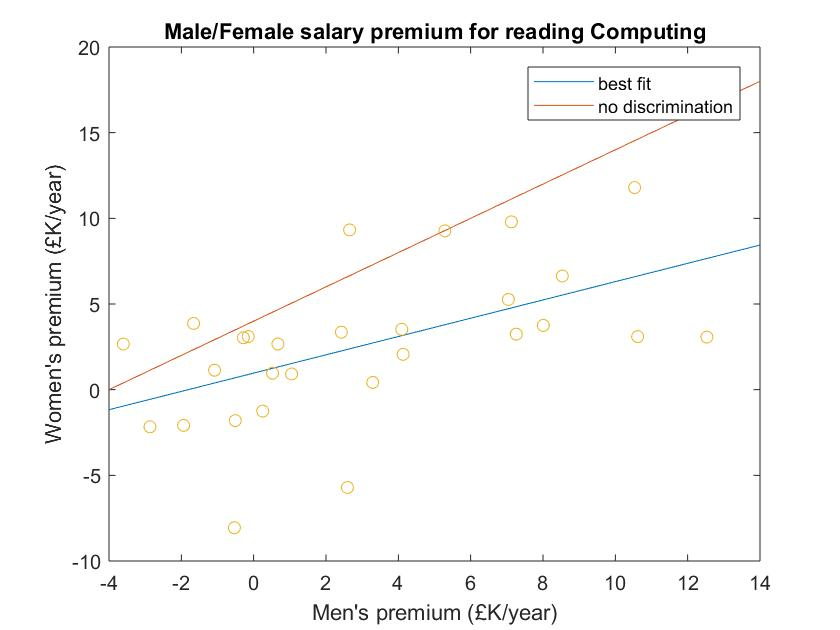
\includegraphics[scale=0.34]{BBCSalaryDatav4.jpg}}
\end{figure}

\section{UK Higher Education Policy Context}\label{ukhepolicy}

It is worth recalling that, after the Government's acceptance of the
Browne report \cite{BIS2010a}, students in England pay probably the
highest\footnote{Or possibly second-highest after US students, but the
US averages in \cite[Table B5.1]{OECD2016a} conceal an enormous
variation.} prices in the world for undergraduate education: between
\pounds6000 and \pounds9000/year for tuition alone. While this is
normally covered by student loans repaid on an income-contingent
basis, essentially through a 9\% income tax premium, there is evidence
\cite{CallenderMason2017a} that this ``contribute[s] to lower rates of
planned H[igher] E[ducation] participation by lower-class students''.

\subsection{Teaching Excellence Framework}
%AH to write overview paragraph. But JHD will try.

UK universities have been judged, very publicly, on their research
for the last thirty years by the Research Assessment Exercise (RAE), and its successor the Research Evaluation Framework (REF). This has led to many complaints, largely justified, that teaching, because it is not measured, is not taken as seriously as research, certainly in some of the research-intensive universities. Similar comments in the USA can be found in \cite{Campbelletal2018a}. To counteract this, the Government introduced (first grades published in June 2017) a `` Teaching Excellence Framework'' (TEF)\footnote{Now renamed ``Teaching Excellence and Student Outcomes Framework'', which is somewhat more descriptive.}. The ostensible aim of the TEF was to evaluate the quality of HE provision for each Higher Education provider within the United Kingdom.
The initial version of the TEF produced a university-wide assessment on a three-point (Gold-26\%/Silver-50\%/Bronze-24\%) scale. It in fact used no assessment of teaching as such, merely statistical data such as that used in \cite{Shadbolt2016a}.

In 2018, following an Institutional-level review undertaken in the previous year, the Office for Students (OFS) conducted a pilot of a national  subject-based TEF. The objective was to provide sufficient data for prospective students to enable them to undertake an informed decision about their choice of University and subject of study. This was particularly pertinent to the UK context as the funding of Higher Education has shifted, following several policy changes, the latest being the
Browne report \cite{BIS2010a}, from students receiving means-tested Government grants to undertaking a loan to pay for their tuition. % Typical tuition fees are set at around £9k per annum.

%Fifty higher education providers participated in the 2018 pilot, reflecting the diverse range of UK HE within the sector. The pilot collated subjects into 7 groups with 142 subject panel members reviewing the provision. The subject panels consisted of members of the academic community, students, employers and representatives of the professional bodies. Reviewing panels rated a HE provider's subject provision as being either Gold, Silver or Bronze. The Computing subject was grouped with Engineering and Technology. The main goal of the pilot was to inform the development of the subject-TEF methodology to be adopted by the national roll-out currently scheduled for 2019/20. The framework evaluated subject-provision against 6 core metrics. Three of these came directly from the National Student Survey (teaching, academic support and assessment and feedback) one for continuation (retention) and two were related to employment (employment or further study/ highly skilled employment or further study). Reviewers are able to review a provider's metrics against a range of indicators %JHD was "stakeholders"
%including full/part-time students, ethnic diversity, gender, age profile etc. Additionally, supplementary statistics are provided to inform the panel members' review. These include teaching intensity (contact hours in all its various guises) and long-term employment/earnings as measured by the Longitudinal Education Outcomes (LEO) data \cite{DfE2017a}.

The TEF's reliance on employment metrics pre-supposes a strong correlation between the quality of provision and the employment prospects/performance of the students. This can be challenging for some disciplines (e.g. income earning potential is not equally distributed across all subjects). The intention however is clear. In the context of students paying their own tuition fees, quality of provision is being linked to future employment prospects. This represents an opportunity for HE Computing provision. Those programmes, characteristic of most in computer science,  that contain a placement/internship, are professionally-accredited and whose curriculum is informed by an employer-led advisory board are well-placed to do well in the TEF. 

\subsection{Degree Apprenticeships}\label{sec:DA}

The Government has also launched ``Degree Apprenticeships''
\cite{BIS2015a}. These were described by the then Prime Minister as
``combining a full degree with the real practical skills gained in
work and the financial security of a regular pay packet''. The
employer pays the tuition cost, but due to the Apprenticeship Levy
\cite{HMRC2016a}, essentially a 0.5\% payroll tax, large (payroll over \pounds3M) employers will find there is no net cost, while smaller employers can claim 90\% of the cost from the Government.

Degree Apprenticeships can be either ``Level 6'' (BSc. level) or ``Level 7'' (MSc. level''). The Level 6 ones last 3--5 years, typically 4. One such is detailed at \url{http://www.aston.ac.uk/study/degree-apprenticeships/employers/degree-apprenticeship-programmes/digital-and-technology-solutions-degree-apprenticeship/}. The Government has yet to approve the details of Level 7 ones, so not much can be said.

\section{Skills mismatch}\label{sec:Skills}

There is a widespread and longstanding complaint that ``students
aren't industry-ready'', or ``there is a skills mismatch''. Some of
this is due to a misapprehension on the part of employers -- and
perhaps misunderstanding of the nature of education versus training
(for example, exhibited by those outside the IT industry itself, but
seeking to hire people with ``10 years experience of programming in
Ruby''), but much of it is genuine. Previous work in this space has
focused on the evidence based for how programming and software
engineering is taught at degree
level~\cite{davenport-et-al:latice2016,murphy-et-al:programming2017,simon-et-al:sigcse2018}. One
of the main challenges for the university community is to better
understand this complaint.

\subsection{Sandwich Years}

In the UK context, a university course that includes a period
working in industry (which may include government, charities, etc.) is
generally called ``sandwich'', and in North America the term ``co-op''
is generally used. The most common model in Computing in England,
where the vast majority of students study three-year Bachelor's
degrees, is a year's placement in industry between the second and
final years of study. This is remarkably successful in computing. The
University of Bath has run such courses since its founding (1966),
with about 80\% of students opting to take the sandwich year. There is
statistical evidence for its success wherever it is used in the
UK\footnote{And at least anecdotal evidence elsewhere: ``the co-op
system is a major reason for our [University of Waterloo] success''
\cite{Watt2017a}.}:

\begin{quote} those studying sandwich courses enjoy the lowest levels
of unemployment (6\% sandwich vs 15\% non-sandwich), the lowest levels
of non-graduate level employment (6\% sandwich vs 25\% non-sandwich),
and graduates from sandwich courses are twice as likely to be earning
over \pounds20,000 compared to those who did a standard
degree. \cite[\P2.5]{Shadbolt2016a}
\end{quote}

A simplistic remedy would be to require that all students study
sandwich degrees, but this has numerous objections:

\begin{enumerate}
\item Some students do not wish to, often for valid reasons;
\item The supply of employers willing to offer such placements is
limited, and often they are only offered to a limited number of
universities with whom the employer has built up relations, often
going back decades;
\item The university needs to invest in the process: a successful
sandwich year programme is not a matter of simply allowing students to
intermit their studies.
\end{enumerate}

Hence we should ask ourselves \emph{why} such courses are so
successful (if indeed they are: there is a possible confounding
factor, in that, for those universities with scanty support for the
sandwich system, those students that do take a sandwich year wil tend
to be the more self-motivated ones, who would probably do well
anyway).  %Thanks to Matt for this!  
There are, it seems to the
authors, two classes of reasons: those intrinsic to the sandwich
process, and the skills the sandwich process confers. The first class
is easy to understand: the employer can view the year as a year-long
assessment phase before deciding whether to offer a permanent
job. Bath's experience is that about 2/3 of sandwich placements result
in job offers to the student. However, it is the second class that we
need to investigate in the hope that non-sandwich courses can learn from them. A major one, brought out repeatedly by students
returning from placement, is team working.

\subsection{Team/Group working}

``Teamwork'' is often identified as a key skill \cite[and many
others]{ArcherDavidson2008}. Simplistically, then, universities should
teach it. Indeed, the British Computer Society has long required this
of degrees it accredits:
\begin{quote} An ability to work as a member of a development team
recognising the different roles within a team and different ways of
organising teams \cite[Requirement 2.3.1]{BCS2018a}.
\end{quote}
The problem is that group working is unpopular with students. Most of
them have never experienced it in their academic work at school, and
really dislike ``being dragged down'', as they generally put it, by
others. In many countries, this wouldn't matter, but the UK has (many
would say ``suffers from'', see, e.g. \cite{Cupples2015a}) the
National Student Survey \cite{OfS2018a}. The results of this, notably
the headline ``are you satisfied with your course'' question, are
pored over intently by university management \cite[Myth
3]{OfS2018a}. As well as the quantitative scores, the students submit
free-text responses, and it does not take many students complaining
about the group work before the Pro-Vice-Chancellor (Teaching) or
equivalent\footnote{Whose pay may well be linked to these scores.} is
beating down the Director of Studies door, saying ``obviously you must
abolish group work immediately''. Both the first and third authors have been Directors of Studies, and can vouch for this.

However, a BCS-accredited course gives the response ``but our accreditation demands it'', whereupon the discussion can evolve into a more sensible debate about the size, shape and process of group working.
\par
This leads to a curious paradox. Employers value group working experience (at a Shadbolt Review focus group, every employer stated they always asked potential employees about experience of group working), group working experience is only taught because accreditation requires it, but employers do not value accreditation.  ``systems of accreditation more broadly are poorly understood and valued by employers, students and HE providers'' \cite[\P2.12]{Shadbolt2016a}.

\subsection{Code Review}\label{sec:Code}
A further aspect of the ``not industry ready'' complaint has recently been identified by the Institute of Coding team as part of the engagement with industry, and is described by a prominent industrialist from the safety-critical sector as follows. 
\begin{quote}
We do find we have to train grads how to review stuff properly --- both personal (their own stuff) and team/peer reviews. While they may have been exposed to the concept of personal and peer reviews, none of them have actually been taught how to do it properly and how to measure its effectiveness. \cite{Chapman2018c}
\end{quote}
This quote is supported by many Institute of Coding industrialists, and also by the work of  \cite{Boerstleretal2018a}, though their conclusion ``Code quality should be discussed more thoroughly in educational programs'' is probably too weak. As \cite{Chapman2018c} says ``While they may have been exposed to the concept of personal and peer reviews'' it is unlikely that many of them will actually have practiced it.  One might ask ``but what about the group working''? 
\par
That is a good question, and one that the Institute of Coding is investigating. A provisional answer lies in the nature of group working. Practically all BCS-accredited universities meet the requirement \cite[Requirement 2.3.1]{BCS2018a} (and ``working with others'' \cite[Requirement 2.3.2]{BCS2018a}) by means of a group practical project. This is practically always done before the final year, both for reasons of balance (BCS also requires an individual project amounting to at least 25\% of the final year \cite[Requirement 2.5.1]{BCS2018a}) and, more pragmatically, so that the memory of this disliked experience will have worn off before the students complete the National Student Survey in their final year. Universities with a strong sandwich programme also want students to be at least engaged on a group project when they go to their interviews.

But students hate being ``dragged down'' by their fellow team-members (it is odd that Directors of Studies and group project lecturers hear far less about being ``dragged up''!).  Hence students are very keen to have ``their own bit'' of the group activity, and it is difficult to have true team responsibility and code reviews.  Various attempts are being made at this, e.g. at Bath the use of ``Agile'' methodology with testing formally built into the  set of sprints, but it is probably fair to say that this is an under-researched area.  \cite{Hundhausenetal2013a} is one of the few pieces of research, but they say ``In future research, we would like to systematically investigate best practices for building effective P[edagogical]C[ode]R[eview] teams''. 

% this is the main section? do we have text to rip from the IoC bid
% doc?
% do we want to add note about nomenclature/terminology -- not hugely happy with
% "Institute of Coding'', but this was political, etc...
\section{Institute of Coding}\label{ioc}

Formally announced in \cite{DfE2018a}, but foreshadowed in
\cite{HMG2015a}, the Institute of
Coding\footnote{\url{https://instituteofcoding.org}} is one of the
UK Government's latest responses to the ``Digital Skills
Challenge''. The Institute brings together a consortium of research-
and teaching-focused universities, large corporates, small- and
medium-sized enterprises (SMEs), established industry groups, experts
in the delivery of distance/non-traditional learning and professional
bodies to develop and deliver innovative, industry-focused education
across the UK. It is explicitly an industry--university collaboration,
with the Government contributing at most 50\% of the money.

It brings together for the first time traditional computer science
departments and business schools, leaders in art and design,
innovation in programme delivery, the industry backing of the UK's
leading digital employers, and the leading professional bodies.  The
Institute's vision is that ``every student leaves education with
employment, and that employers and individuals across the UK have
ready access to the skills they need to compete successfully in the
global digital economy''. It is structured around five themes.

\subsection{``University Learners''}

This is aimed at understanding, and solving, the ``Skills Mismatch''
problems (see \S\ref{sec:Skills}). As seen from \S\ref{sec:Code},
these problems can be quite subtle, and are not addressed by such broad
requirements as \cite[Requirement 2.3.1]{BCS2018a}.  Hence the
Institute is also looking at accreditation, with a view to producing
more detailed records, essentially e-portfolios, of skills
achieved. It is possible that these will be supported by a
blockchain-based mechanism, as is being done elsewhere
\cite{RMIT2018a}.

\subsection{``The Digital Workforce''}

In practice this is largely aimed at degree apprenticeships (see
\S\ref{sec:DA}). These are still in their very early days in
computing, and we hope that the Institute will enable best practice
sharing from the beginning. In terms of content, as opposed to
pedagogic practice, this theme is tightly linked with theme 1, notably
in areas like CyberSecurity, where there is a great shortage of
non-proprietary teaching material.

\subsection{``Digitalising the Professions''}

The official description ``to transform professions undergoing digital
transformation'' \cite{DfE2018a} is tautologous, but the consortium
aims are to provide a flexible modular digital masters programme aimed
at people in various professions where digital technologies are
changing the job such that serious upskilling in necessary, and also
to provide various short taster courses in order to widen the reach of
digital skills. As for theme 2, this will be sharing content with theme 1.

\subsection{``Widening Participation''}

This is aimed at the problems identified in \S\ref{sec:Gender}. Since
the Institute bid was submitted, the salary data in \cite{DfE2018d}
(see Figure \ref{fig:BBC}) have been released, which show the
importance of a more nuanced study of the effect of gender in
particular. The analysis in \cite{DfE2018d} concentrated on gender,
but we are hoping to do similar studies for computer science with
regard to other characteristics such as ethnicity.

\subsection{``Knowledge Sharing and Sustainability''}

A perverse, but totally natural, consequence of the REF has been the
marginalisation of pedagogy research in the UK
\cite{Cottonetal2018a}. This is particularly acute in Computing, and
can be quantified by noting that Australia, with less than 40\% of the
population of the UK, sends practically the same number of papers to
the Koli Calling conference in Finland as the UK does
\cite{Simon2016a}. Dissemination of good practice is also low:
\cite{murphy-et-al:programming2017} was the first survey of its kind
in the UK, despite the fact that they had been running for many years
elsewhere \cite{simon-et-al:sigcse2018}.

Delivering as much education as the Institute proposes presumes a
supply of educators; this is a major challenge at all levels for
computing in the UK~\cite{brown-et-al:toce2014}, as it is in many
countries. We have seen a number of challenges in the recruitment and
retention of teachers 
%(especially in  England~\cite{sentance+waite:2018}), as well as issues with effectively scaling professional development opportunities~\cite{sentance+csizmadia:2017} (for example, subject knowledge enhancement, pedagogic knowledge, as well 
and funding to
access courses and higher degree
programmes~\cite{sentance-et-al-wipsce2012}).  Hence one workpackage
in this theme is devoted to ``educating the educators''

A further challenge is sustainability. The Government funding for the
Institute is very short-term, and indeed will lapse before anyone
graduates from a Level 6 (BSc.)  degree apprenticeship. Hence the
Institute needs to become self-supporting in a very short timeframe.


% From CfP:
% Short papers (up to 5 pages) focus on dissemination and discussion
% of new ideas in computing education practice or research that merit
% wider awareness and discussion within the community. They can present
% preliminary results of new educational innovations...

% TC: so are we going to talk about the IoC "national" model, with
% industry matched funding, etc?

\section{Impact to date}
The Institute of Coding is very much ``work in progress'': at the time
of writing it was less than nine months old.  The mere adumbration
\cite{HMG2015a} prompted the research in
\cite{murphy-et-al:programming2017}, and the various working groups
round the themes are causing more discussion of computing pedagogy in
the UK than the authors can ever remember, further reinforced by the
recommendations in~\cite{rs:2017}.  

There are new courses already started, or planned to start in 2019, badged as ``Institute of Coding'', mostly Degree Apprenticeships, Masters courses, or joint Masters courses and (level 7) Degree Apprenticeships.  It could be argued that some, particularly the Degree Apprenticeships, might have been started without the Institute of Coding, but it is certainly the case that the Institute of Coding has accelerated the process, not least by short-circuiting the often labyrinthine ``quality assurance'' processes in universities, as university leadership, prompted by the money on offer, had already signed up to the principle. 

\section{Future Work and Replicability}\label{concl}

We are now seeing a number of successful initiatives, activities and
interventions which may prove useful to other nations reforming their
curricula (both compulsory, school-level, as well as post-compulsory),
as well as in the wider aim of developing broader -- sustainable and
transferable -- societal digital skills. However, we recognise that
there has been a significant corpus of work in this space, with a
multitude of initiatives and activities purporting to fix the problem;
it is thus important not to repeat past failures.

When establishing a model for viewing school computer science
education, it is apparent that there is substantial diversity between
education systems -- from formal school curricula through to tertiary
education, as well as wider education policy and funding -- and this
can create obstacles when trying to understand progress made in one
country and potentially replicate it in
another~\cite{hubwieser:2013}. This is particularly relevant to the
devolved (and diverging) educational systems of the UK, as well as the
variety of its disparate interventions, especially formal curricula
and post-compulsory/tertiary education.  There remain significant
challenges, particularly around connectedness and coherency of policy,
as well as bridging the gap between the expectations and evolving
requirements of (higher) education and industry.


However, two overarching themes are apparent; firstly, such effort has
to be viewed as a coordinated multi-pronged approach, requiring an
overarching holistic strategy, working collaboratively with
universities, colleges, employers including but not limited to
industry, local and national government, as well as young people,
parents and the wider public. Secondly, there is a need to overcome
the challenges of recurrent funding and support to ensure long-term
sustainability of the interventions --- across the four nations of the
UK --- as well as ensuring parity of opportunity for all young
learners. Whilst we do not necessarily recommend replicating some of
the policy structures under which the UK operates, especially national
quality assessment exercises such as the TEF, they can provide a
useful policy lever for initiatives such as the Institute.

The Institute of Coding could thus provide a national cohering role,
collaborating with other organisations working on school-level
interventions (such as Computing At School (CAS), Raspberry Pi
Foundation, Technocamps, {\it et al\/}.), providing a platform for
conducting research activities; building the evidence base and
informing policy; supporting accreditation and standards; as well as
changing the wider perception -- and economic, societal and cultural
importance -- of `ICT', `digital', `coding' and other cognate areas.

\section*{Acknowledgements}

This work was supported by the Institute of Coding which received
\pounds20m of funding from the Office for Students (OfS), as well as
support from the Higher Education Funding Council for Wales (HEFCW).
\ifanon
%The first author is grateful to Matt Dickson (University of Bath) for discussions about \cite{DfE2018d}, but any mistakes are the authors' alone.
\fi

\bibliographystyle{ACM-Reference-Format}
\bibliography{ACMCompEd2019} 

\end{document}
